% Overleaf-ready LaTeX document for Campus Compass 360
\documentclass[11pt,a4paper]{article}
\usepackage[margin=1in]{geometry}
\usepackage{hyperref}
\usepackage{graphicx}
\usepackage{array}
\usepackage{longtable}
\usepackage{titlesec}
\usepackage{enumitem}
\usepackage{caption}
\usepackage{booktabs}
\usepackage{tikz}
\usetikzlibrary{arrows.meta, positioning, shapes.multipart, calc}

\hypersetup{
  colorlinks=true,
  linkcolor=blue,
  urlcolor=blue,
  citecolor=blue
}

\title{Campus Compass 360\\System Analysis and Design}
\author{}
\date{\today}

\begin{document}
\maketitle

\section{Overview}
Campus Compass 360 is a web application that provides an immersive virtual campus tour using 360-degree panoramas and a complementary map viewing mode. It integrates AI-driven tour recommendations, user reviews, and an administrative interface for managing locations and media.

The platform uses:
\begin{itemize}[leftmargin=1.4em]
  \item Next.js (App Router), React, TypeScript
  \item Tailwind CSS, ShadCN UI
  \item Supabase (Auth, Postgres with RLS, Storage; Realtime optional)
  \item Photo Sphere Viewer (\texttt{@photo-sphere-viewer/core})
\end{itemize}

\section{Goals and Scope}
\subsection*{Goals}
\begin{itemize}[leftmargin=1.4em]
  \item Provide a seamless 360° campus exploration experience.
  \item Allow non-technical admins to manage locations and media.
  \item Recommend personalized tours via AI.
  \item Enable users to review locations and save tours.
\end{itemize}

\subsection*{Out of Scope}
\begin{itemize}[leftmargin=1.4em]
  \item Indoor mapping and real-time indoor positioning.
  \item Complex GIS integration beyond static map images.
\end{itemize}

\section{Stakeholders}
\begin{longtable}{@{}p{0.24\linewidth} p{0.72\linewidth}@{}}
\toprule
\textbf{Stakeholder} & \textbf{Interests} \\\midrule
Prospective Students & Explore campus, discover points of interest. \\
Current Students     & Navigate campus, review locations. \\
Administrators       & Manage locations, ensure data integrity and security. \\
Engineering Team     & Maintain scalability, reliability, and developer productivity. \\\bottomrule
\end{longtable}

\section{Functional Requirements (Summary)}
\begin{itemize}[leftmargin=1.4em]
  \item 360° Viewer: pan/zoom, hotspots for navigation, optional auto-rotate.
  \item Map Viewer: multiple images, zoom/pan, fullscreen, keyboard controls.
  \item AI Tours: interest-based recommendations; save tours to profile.
  \item Reviews: authenticated users can rate/comment; all can read.
  \item Admin: CRUD locations, upload panoramas/thumbnails to Supabase Storage.
\end{itemize}
See \texttt{src/docs/REQUIREMENTS.md} for a complete list.

\section{System Context}
\begin{center}
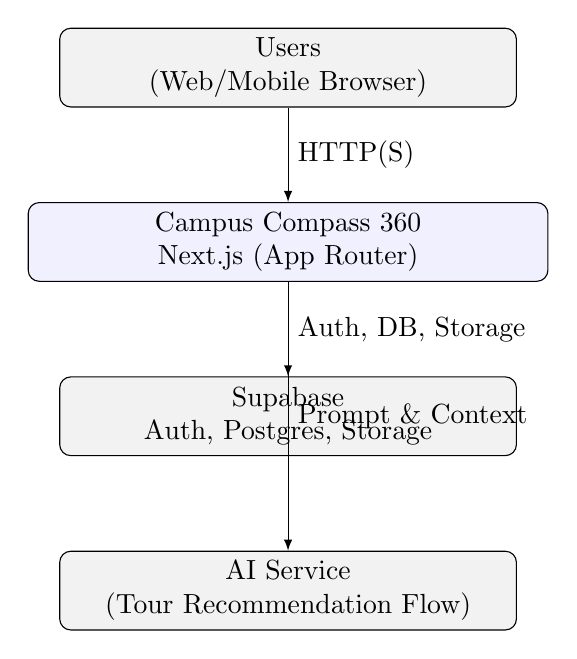
\begin{tikzpicture}[>=latex, node distance=1.2cm]
  \tikzstyle{ext}=[draw, rounded corners, align=center, minimum width=5.8cm, minimum height=1.0cm, fill=gray!10]
  \tikzstyle{sys}=[draw, rounded corners, align=center, minimum width=6.6cm, minimum height=1.0cm, fill=blue!6]

  % Vertical layout
  \node[ext] (user) {Users\\(Web/Mobile Browser)};
  \node[sys, below=1.2cm of user] (app) {Campus Compass 360\\Next.js (App Router)};
  \node[ext, below=1.2cm of app] (supabase) {Supabase\\Auth, Postgres, Storage};
  \node[ext, below=1.2cm of supabase] (ai) {AI Service\\(Tour Recommendation Flow)};

  \draw[->] (user) -- node[midway, right]{HTTP(S)} (app);
  \draw[->] (app) -- node[midway, right]{Auth, DB, Storage} (supabase);
  \draw[->] (app) -- node[midway, right]{Prompt \& Context} (ai);
\end{tikzpicture}
\end{center}

\section{High-Level Architecture}
\subsection*{Frontend}
\begin{itemize}[leftmargin=1.4em]
  \item Next.js App Router with client and server components.
  \item Route Handlers under \texttt{src/app/api/*} for Postman testing.
  \item Client providers for Supabase; custom hooks for auth and data.
  \item 360° viewer and map viewer as client components.
\end{itemize}

\subsection*{Backend (Supabase)}
\begin{itemize}[leftmargin=1.4em]
  \item Postgres tables: \texttt{users}, \texttt{locations}, \texttt{saved\_tours}, \texttt{reviews}.
  \item RLS policies enforce least privilege (see Sec.~\ref{sec:security}).
  \item Storage bucket \texttt{locations} (public) serves panoramas and thumbnails.
  \item Realtime subscriptions optional and fail-safe.
\end{itemize}

\section{Use Cases}
\begin{longtable}{@{}p{0.20\linewidth} p{0.76\linewidth}@{}}
\toprule
\textbf{UC-1: Explore 360°} & User pans/zooms panoramas, clicks hotspots to navigate. \\\midrule
\textbf{UC-2: View Map} & User switches to map mode, browses images, zooms/pans. \\\midrule
\textbf{UC-3: Login/Signup} & User authenticates with email/password (Supabase Auth). \\\midrule
\textbf{UC-4: AI Tour} & User enters interests; system returns a recommended tour. \\\midrule
\textbf{UC-5: Save Tour} & Authenticated user saves tour for later. \\\midrule
\textbf{UC-6: Reviews} & Authenticated user posts rating/comment; all users view. \\\midrule
\textbf{UC-7: Admin CRUD} & Admin creates/updates/deletes locations and uploads media. \\\bottomrule
\end{longtable}

\section{Key Sequence Diagrams}
\subsection*{AI Tour Recommendation}
\begin{center}
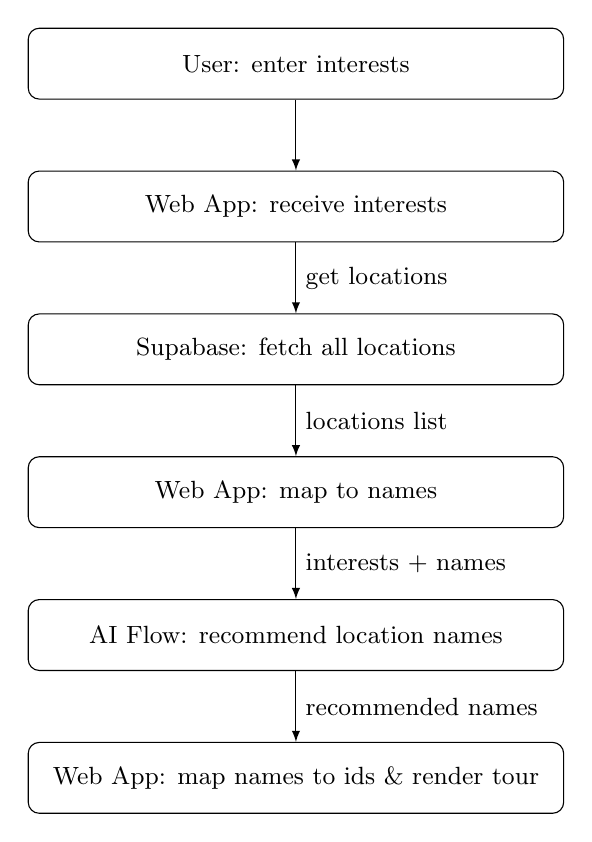
\begin{tikzpicture}[node distance=0.9cm, >=latex, font=\small]
  \tikzstyle{stepnode}=[draw, rounded corners, align=center, minimum width=6.8cm, minimum height=0.9cm, fill=white]

  % Vertical sequence (top -> bottom)
  \node[stepnode] (u) {User: enter interests};
  \node[stepnode, below=0.9cm of u] (w1) {Web App: receive interests};
  \node[stepnode, below=0.9cm of w1] (s1) {Supabase: fetch all locations};
  \node[stepnode, below=0.9cm of s1] (w2) {Web App: map to names};
  \node[stepnode, below=0.9cm of w2] (ai) {AI Flow: recommend location names};
  \node[stepnode, below=0.9cm of ai] (w3) {Web App: map names to ids \& render tour};

  \draw[->] (u) -- (w1);
  \draw[->] (w1) -- node[right]{get locations} (s1);
  \draw[->] (s1) -- node[right]{locations list} (w2);
  \draw[->] (w2) -- node[right]{interests + names} (ai);
  \draw[->] (ai) -- node[right]{recommended names} (w3);
\end{tikzpicture}
\end{center}

\subsection*{Admin Adds Location}
\begin{center}
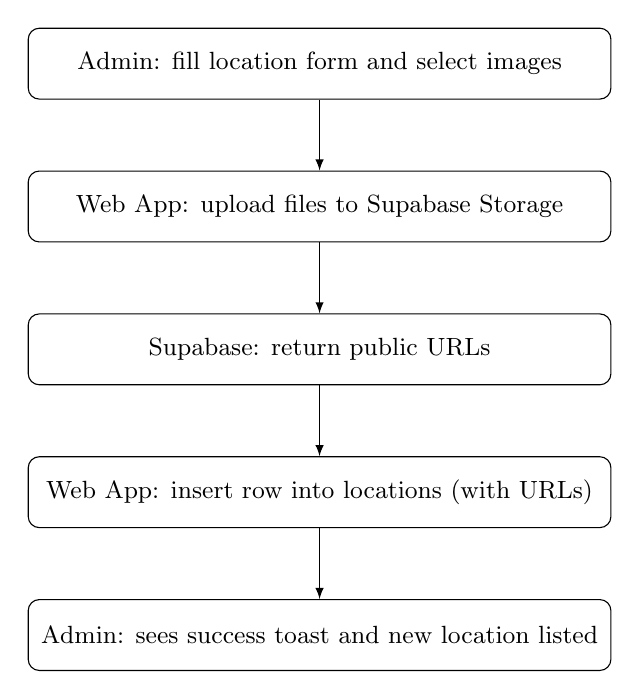
\begin{tikzpicture}[node distance=0.9cm, >=latex, font=\small]
  \tikzstyle{stepnode}=[draw, rounded corners, align=center, minimum width=7.4cm, minimum height=0.9cm, fill=white]

  \node[stepnode] (a1) {Admin: fill location form and select images};
  \node[stepnode, below=0.9cm of a1] (w1) {Web App: upload files to Supabase Storage};
  \node[stepnode, below=0.9cm of w1] (s1) {Supabase: return public URLs};
  \node[stepnode, below=0.9cm of s1] (w2) {Web App: insert row into locations (with URLs)};
  \node[stepnode, below=0.9cm of w2] (a2) {Admin: sees success toast and new location listed};

  \draw[->] (a1) -- (w1);
  \draw[->] (w1) -- (s1);
  \draw[->] (s1) -- (w2);
  \draw[->] (w2) -- (a2);
\end{tikzpicture}
\end{center}

\section{Data Model}
\subsection*{Tables}
\begin{itemize}[leftmargin=1.4em]
  \item \textbf{users(uid PK)}: email, display\_name, photo\_url, is\_admin, created\_at, last\_login
  \item \textbf{locations(id PK)}: name, description, panorama\_url, thumbnail\_url, coordinates(jsonb), connections(jsonb), created\_at, updated\_at
  \item \textbf{saved\_tours(id PK)}: user\_id FK(users.uid), name, description, location\_ids(text[]), created\_at
  \item \textbf{reviews(id PK)}: location\_id FK(locations.id), user\_id FK(users.uid), display\_name, rating, comment, created\_at
\end{itemize}
See \texttt{src/docs/backend.json} for details.

\section{Security and RLS}\label{sec:security}
\subsection*{Authentication}
Supabase Auth with email/password. Client-side uses a custom hook to fetch the verified user via \texttt{auth.getUser()}.

\subsection*{Authorization (RLS)}
\begin{itemize}[leftmargin=1.4em]
  \item \textbf{locations}: \emph{SELECT} for all; \emph{INSERT/UPDATE/DELETE} only for admins (\texttt{users.is\_admin = true}).
  \item \textbf{users}: users can \emph{SELECT/UPDATE} only their own row (\texttt{uid = auth.uid()}).
  \item \textbf{saved\_tours}: a user can \emph{ALL} only for rows where \texttt{user\_id = auth.uid()}.
  \item \textbf{reviews}: public \emph{SELECT}; \emph{INSERT/UPDATE/DELETE} only where \texttt{user\_id = auth.uid()}.
\end{itemize}

\section{API Design (Testing)}
HTTP endpoints are exposed via Next.js route handlers for Postman:
\begin{itemize}[leftmargin=1.4em]
  \item Auth: \texttt{POST /api/auth/signup}, \texttt{/login}, \texttt{/logout}
  \item Actions: \texttt{POST /api/actions/getTourRecommendations}, \texttt{/saveTour}, \texttt{/addReview}, \texttt{/addLocation}; \texttt{PUT /api/actions/updateLocation}; \texttt{DELETE /api/actions/deleteLocation}
  \item Queries: \texttt{GET /api/locations}, \texttt{GET /api/reviews?location\_id=\{id\}}, \texttt{GET /api/tours}
\end{itemize}

\section{Non-Functional Requirements}
\begin{itemize}[leftmargin=1.4em]
  \item \textbf{Performance}: Optimized initial load; viewer must remain smooth.
  \item \textbf{Security}: All server actions verify auth via \texttt{getUser()}; RLS enforces row-level access.
  \item \textbf{Reliability}: Realtime subscriptions are optional; system remains functional without them.
  \item \textbf{Maintainability}: Clear module boundaries; typed APIs; provider/hooks for Supabase.
\end{itemize}

\section{Deployment}
\begin{itemize}[leftmargin=1.4em]
  \item Frontend: Next.js build on Vercel or similar.
  \item Backend: Supabase project (managed Postgres \& Storage).
  \item Environment: \texttt{NEXT\_PUBLIC\_SUPABASE\_URL}, \texttt{NEXT\_PUBLIC\_SUPABASE\_ANON\_KEY}, optional \texttt{NEXT\_PUBLIC\_ENABLE\_REALTIME=false}.
\end{itemize}

\section{Risks and Mitigations}
\begin{itemize}[leftmargin=1.4em]
  \item \textbf{Large Media}: Use thumbnails, CDN, and lazy loading.
  \item \textbf{Auth Drift}: Always use \texttt{auth.getUser()} server-side to verify identity.
  \item \textbf{Realtime Noise}: Disable or guard subscriptions; manual refetch available.
  \item \textbf{RLS Misconfig}: Keep policies version-controlled; test with Postman.
\end{itemize}

\end{document}


